\documentclass[11pt,letterpaper,twoside,openright]{report}
\usepackage[utf8]{inputenc}
\usepackage[english]{babel}

%preámbulo configuración de página
\usepackage[width=165mm,top=15mm,bottom=25mm,bindingoffset=20mm,includehead]{geometry}

%Preámbulo de Color de texto =================================================================
\usepackage{color}
\definecolor{gray97}{gray}{.97}
\definecolor{gray75}{gray}{.75}
\definecolor{gray45}{gray}{.45}
\definecolor{verde}{rgb}{0.0, 0.5, 0.0}

%preámbulo captions==========================================================================
\usepackage{caption}
\captionsetup{margin=40pt,format=hang,indention=-.5cm,font={footnotesize, rm},labelfont=bf,labelsep=colon}

%preámbulo encabezados=======================================================================
\usepackage{fancyhdr}
\pagestyle{fancy}
\fancyhead{}
\fancyfoot{}
\fancyhead[RO,LE]{\thepage}
\fancyhead[LO]{\nouppercase{\rightmark}}
\fancyhead[RE]{\nouppercase{\leftmark}}
\setlength{\headheight}{15pt} 


%preámbulo matemáticas=======================================================================
%\spanishdecimal{.}
\usepackage{amsmath}
\usepackage{amsfonts}
\usepackage{amssymb}
\usepackage{amsthm}
\usepackage{dsfont}
\usepackage{mathrsfs}
\newcommand{\sign}[1]{\mathrm{sign(#1)}} 
\newcommand{\refe}[1]{(\ref{#1})}
\newcommand{\rojo}[1]{{\color{red} #1}}
\newcommand{\RE}{\mathbb{R}}
\newcommand{\sig}[2]{\lceil#1\rfloor^{#2}}
\newcommand{\abs}[2]{|#1|^{#2}}
\providecommand{\norm}[1]{\lVert#1\rVert}
\usepackage{color}   
\setcounter{MaxMatrixCols}{20}
%\decimalpoint


%preámbulo sistema internacional de unidades================================================
\usepackage{siunitx}


%preámbulo referencias========================================================================
\usepackage[numbers]{natbib}
%\bibliographystyle{plainnat}
\usepackage[hidelinks, breaklinks=true, backref=page,colorlinks=true,linkcolor=blue,citecolor=magenta]{hyperref}


%preámbulo de gráficos=========================================================================
\usepackage{graphicx}
\graphicspath{{figuras/}}
\usepackage{subfigure}
\usepackage{float}

%Preámbulo tabla=============================================================================
\usepackage{multirow, array}
\usepackage{booktabs}
\usepackage{colortbl}
\definecolor{SeaGreen}{rgb}{0.13, 0.7, 0.67}
\definecolor{Peach}{rgb}{0.97, 0.51, 0.47}
\definecolor{LimeGreen}{rgb}{0.31, 0.78, 0.47}
\definecolor{bananayellow}{rgb}{1.0, 0.88, 0.21}
%preámbulo de apéndices======================================================================
\usepackage[toc,page]{appendix}
\renewcommand{\appendixpagename}{Apéndices}

%preámbulo de url============================================================================
\usepackage{url}

%preámbulo de nomenclatura==================================================================
\usepackage[intoc,spanish]{nomencl}
\makenomenclature
\usepackage{etoolbox}


%Preámbulo para código de programación=======================================================
\usepackage{listings}
\lstset{ 
	backgroundcolor=\color{white},
	rulesepcolor=\color{black},
	%
	stringstyle=\ttfamily,
	showstringspaces = false,
	basicstyle=\footnotesize\ttfamily,
	commentstyle=\color{gray45},
	keywordstyle=\bfseries,
	%
}
\renewcommand{\lstlistingname}{Listado}

%Preámbulo numeros decimales================================================================
%\spanishdecimal{.}


%preámbulo Marcadores=======================================================================
\usepackage[hidelinks, breaklinks=true, backref=page]{hyperref} 

%Redifiniendo Titulos==========================================================================
\usepackage{titlesec}
\newcommand{\bigrule}{\titlerule[0.5mm]}
\titleformat{\chapter}[display] % Se cambia el formato del capitulo
%{\bfseries\Huge} % por defecto se usarán caracteres de tamaño \Huge en negrita
{\bfseries\Huge} % por defecto se usarán caracteres de tamaño \Huge en negrita
{% contenido de la etiqueta
	\titlerule % línea horizontal
	\filright % texto alineado a la derecha
	\Large\chaptertitlename\ % "Capítulo" o "Apéndice" en tamaño \Large en lugar de \Huge
	\Large\thechapter} % número de capítulo en tamaño \Large
{0mm} % espacio mínimo entre etiqueta y cuerpo
{\filright} % texto del cuerpo alineado a la derecha
[\vspace{0.5mm} \bigrule] % después del cuerpo, dejar espacio vertical y trazar línea horizontal gruesa

%Preámbulo utilidades=========================================================================
\usepackage{pdfpages}	%Incluye hojas de de archivos PDF
\usepackage{siunitx}			%Sitema internacional de unidades
\usepackage[T1]{fontenc}	%Fuentes
\usepackage{textcomp}		%Fuentes

%preámbulo teoremas, Definiciones y Proposiciones ==============================================================================================================
\newtheorem{theorem}{Theorem}[chapter]
\newtheorem{definition}{Definition}[chapter]
\newtheorem{proposition}{Proposition}[chapter]
\newtheorem{observation}{Observation}[chapter]
\newtheorem{lemma}{Lemma}[chapter]
\newtheorem{property}{Property}[chapter]
\newtheorem{assumtion}{Assumption}[chapter]
\newtheorem{corollary}{Corollary}[chapter]

%preámbulo acronimo ===================================================
\usepackage{acronym}
\acrodef{fl}[FL]{Función de Lyapunov} \acused{fl}
\acrodef{pd}[p.d.]{positiva definida}
\acrodef{ae}[AE]{asintóticamente estable}
\acrodef{gae}[GAE]{global y asintóticamente estable}


%preámbulo de nomenclatura ==========================================
%\usepackage[intoc, spanish]{nomencl}
\makenomenclature
\nomenclature{$MCC$}{Modo de conducción continua}
%FIN DEL PREÁMBULO===================================================

%====================================================================
%====================================================================
%                    INICIO DEL DOCUMENTO
%====================================================================
%====================================================================
\begin{document}
	\chapter{Bl-Homogeneous observers for MIMO linear time invariant systems}
	In this chapter we present the second part of main result in this work. We introduce the design of Bl-homogeneous observers for MIMO-LTI systems assuming strong observability. The idea is to transform the system in to a Special Coordinate Basis, (detailed in Chapter 2) obtaining a representation of the system without need to have a triangular structure. That is, despite the fact that such a triangular restructuring of the system in that special way is a great feature of linear systems and greatly simplifies the convergence analysis. Here, it is shown that the designed observers are able to deal with a more general type of interconnections between subsystems. 
	
	Here we use directly a discontinuous nonlinear observer instead of differentiators. This fact suppress the necessity of using a cascade scheme composed by a linear observer and a discontinuous differentiator.
	
	As in SISO case, the nonlinear injection terms can be designed to accelerate the convergence as much as we want by selecting appropriate and sufficiently large gains. Even more, due to the assignability of bl-homogeneous degrees in the observer we can reach and assure exactly and finite-time (or moreover fixed-time) estimation of the states in presence of unknown inputs.
	
\section{Unknown input observers for LTI-MIMO systems}
Consider the MIMO-LTI system without feedthrough (for simplicity) given by
\begin{equation}
	\begin{split}\label{ecu: CH4 Sys MIMO orig}
	\Sigma: \left\{
	\begin{array}{rl}
		\dot{x} &= Ax + D\omega\\
		y&=Cx
	\end{array}
	\right. \\
	\end{split}
\end{equation}
where $x \in \RE^n$ is the state vector, $\omega \in \RE^m$ the unknown input vector and $y \in \RE^p$ is the output vector. Accordingly, the matrices $A,D,C$ have appropriate dimensions. For simplicity in the development we do not consider a known input $u$, since it does not modify the (observability) properties and it is simple to include it in the observer design. The equations are understood in the Filippov sense \cite{Filipov1988} in order to provide for the possibility to use discontinuous signals in observers. Note that Filippov solutions coincide with the usual solutions, when the right-hand sides are continuous.

The task is to build an unknown input observer (UIO) providing for finite-time (preferably fixed-time convergent and exact) estimation of the states in presence of the unknown inputs. In chapter 2 we have stated the necessary and sufficient conditions for the existence and of UIO. We assume to have strong observability only.

Special Coordinated Basis is a useful tool to represent a system in an appropriate form, see Section 2.XX. to more details.

%Another characterization for strongly observable LTI systems in terms of the relative degree with respect to the unknown input was introduced in \cite{Fridman2006}.
%
%\begin{definition}
%	Following \cite{Isidori1996} the relative degree of system \eqref{ecu: Sys siso orig} with respect to the unknown input is the number $r$ such that
%	\begin{equation}
%		CA^jD=0. \quad j=1,...,r-2, \quad CA^{r-1}D \neq 0
%	\end{equation}
%\end{definition}
%Since the system \eqref{ecu: Sys siso orig} is assumed to be observable (in absence of unknown input), i.e. the matrix 
%
%\begin{equation}
%	\mathcal{O} = \begin{bmatrix}
%		C \\
%		CA \\
%		\vdots \\
%		CA^{n-1}
%	\end{bmatrix}
%\end{equation}
%
%has full rank. Then we can transform the system to the observability canonical form through the state transformation $T=\mathcal{O}^{-1}$, such that the matrices $A,D,C$ take the form

\subsection{Unknown Input Observer design}
Given a strong observable system $\Sigma$ in \eqref{ecu: CH4 Sys MIMO orig} under SCB transformation detailed in Section 2.1, if we take into account the Property 2.XX, then the transformed system $\Sigma_{SCB}(\Sigma_b,\Sigma_d)$ is described by the following set of equations.

Each subsystem $\Sigma_{b,\iota}$ with associated states $x_{b,\iota}\in \RE^{n_{b,\iota}}, \iota=1,...,p_b$ 
\begin{equation}
	\begin{split}\label{ecu: CH4 Sigma_b}
		\Sigma_{b,\iota}: \left\{
		\begin{array}{rl}
		\dot{x}_{b,\iota,1} &= x_{b,\iota,2} + H_{bd,\iota,1}y_d, \quad y_{b,\iota}=x_{b,\iota,1}, \\
		\dot{x}_{b,\iota,j} &= x_{b,\iota,j+1} + H_{bd,\iota,j}y_d, \\
		& \vdots \quad j=1,...,n_{b,\iota}-1\\
		\dot{x}_{b,\iota,n_{b,\iota}} &= A_{bb,\iota}x_{b} + H_{bd,\iota,n_{b,\iota}}y_d, 
	\end{array}
\right. \\
	\end{split}
\end{equation}
moreover $\sum_{\iota=1}^{p_b}n_{b,\iota}=n_b$.

And each subsystem $\Sigma_{d,i}$ with associated states $x_{d,i} \in \RE^{n_{d,i}}, i=1,...,p_d$ 
\begin{equation}
	\begin{split}\label{ecu: CH4 Sigma_d}
		\Sigma_{d,i}: \left\{
		\begin{array}{rl}
		\dot{x}_{d,i,1} &= x_{d,i,2} + H_{dd,i,1}y_d,  \quad y_{d,i} = x_{d,i,1} \\
		\dot{x}_{d,i,j} &= x_{c,i,j+1} + H_{dd,i,j}y_d, \\
		& \vdots \quad j=1,...,n_{d,i}-1\\
		\dot{x}_{d,i,n_{d,i}} &= A_{db,i}x_b + A_{dd,i}x_d + w_{d,i}(t),
	\end{array}
\right. \\ 
	\end{split}
\end{equation}
similarly $\sum_{i=1}^{p_d}n_{d,i}=n_d$.

Where $A_{bb,\iota},H_{bd,\iota,j},A_{dd,i},A_{db,i},H_{dd,i,j}$ are constant row vectors of appropriate dimensions. Recall that $\Sigma_b$ corresponds to the observable dynamics of the system, and $\Sigma_d$ with presence of unknown inputs corresponds to the strong observable dynamics. It is clear that $\Sigma_b$ can be expressed in observer or observability  canonical form, the first one allow us to apply directly and homogeneous differentiator as an observer\cite{Niederwieser2021}, but it can not be applied in the observability form. On the other hand, the idea of this work is to show that observers with bl-homogeneous terms can deal with this kind of structures.

\begin{assumtion}\label{Assum: CH4 omega}
	Unknown input $\omega(t)$ a is uniformly bounded function $\norm{\omega(t)}\leq \Delta$, i.e. each element of the vector $|w_{d,i}(t)|< \Delta_{i} \in \mathbb{R}_{\geq 0}$
\end{assumtion}
This allow us to relax the existence conditions of UIO in other to have an observer under strong observability only, see ($**$section 2.x). The relative degree of the outputs $y_{d,i}$ with respect to the unknown input is $n_{d,i}$.

The observer $\Omega(\Omega_b,\Omega_D)$ is given by
\begin{equation}
	\begin{split}\label{ecu: CH4 Omega_b}
		\Omega_{b,\iota}: \left\{
		\begin{array}{rl}
			\dot{\hat{x}}_{b,\iota,1} &= -k_{b,\iota,1}L \tilde{\phi}_{b,\iota,1}( \hat{x}_{b,\iota,1}-y_{b,\iota} ) + \hat{x}_{b,\iota,2} + H_{bd,\iota,1}y_d \\
			\dot{\hat{x}}_{b,\iota,j} &= -k_{b,\iota,j}L^{j} \tilde{\phi}_{b,\iota,j}( \hat{x}_{b,\iota,1}-y_{b,\iota} ) + \hat{x}_{b,\iota,j+1} + H_{bd,\iota,j}y_d  \\
			\vdots \quad & j=1,...,n_{b,\iota}-1\\
			\dot{\hat{x}}_{b,\iota,n_{b,\iota}} &= -k_{b,\iota,n_{b,\iota}}L^{n_{b,\iota}} \tilde{\phi}_{b,\iota,n_{b,\iota}}( \hat{x}_{b,\iota,1}-y_{b,\iota} ) + A_{bb,\iota}\hat{x}_{b}  + H_{bd,\iota,n_{b,\iota}}y_d 
		\end{array}
		\right. \\
	\end{split}
\end{equation}
\begin{equation}
	\begin{split}\label{ecu: CH4 Omega_d}
		\Omega_{d,i}: \left\{
		\begin{array}{rl}
			\dot{\hat{x}}_{d,i,1} &= -k_{d,i,1}L \tilde{\phi}_{d,i,1}( \hat{x}_{d,i,1}-y_{d,i} ) + \hat{x}_{d,i,2} + H_{dd,i,1}y_d,  \\
			\dot{\hat{x}}_{d,i,j} &= -k_{d,i,j}L^{j}\tilde{\phi}_{d,i,j}( \hat{x}_{d,i,1}-y_{d,i} ) + \hat{x}_{d,i,j+1} + H_{dd,i,j}y_d,\\
			\vdots \quad & j=1,...,n_{d,i}-1\\
			\dot{\hat{x}}_{d,i,q_i} &= -k_{d,i,q_i}L^{n_{d,i}} \tilde{\phi}_{d,i,q_i}( \hat{x}_{d,i,1}-y_{d,i} ) + A_{db,i}\hat{x}_b + A_{dd,i}\hat{x}_d
		\end{array}
		\right. \\
	\end{split}
\end{equation}
with positive external gains $k_{b,\iota,j}>0,k_{d,i,j}$ and positive tuning gains $\alpha>0,L >0$, appropriately selected as it will be show latter. 

\newpage
The nonlinear output injection terms $\tilde{\phi}_{b,\iota,j}(\cdot)$ are obtained from the functions

\begin{equation}\label{ecu: CH4 Injection Sigma_b}
	\phi_{b,\iota,j}(s) = \kappa_{b,\iota j} \sig{s}{\frac{r_{(b,\iota),0,j+1}}{r_{(b,\iota),0,1}}} + \theta_{b,\iota j} \sig{s}{\frac{r_{(b,\iota),\infty,j+1}}{r_{(b,\iota),\infty,1}}}
\end{equation}
by scaling the positive internal gains $\kappa_{b,\iota j}>0,\theta_{b,\iota j}>0$
\begin{equation}
	\kappa_{b,\iota j} \rightarrow \left( \frac{L^{n_{b,\iota}}}{\alpha}\right)^{\frac{jd_0}{r_{(b,\iota),0,1}}}\kappa_{b,\iota j} ,\qquad \theta_{b,\iota j} \rightarrow \left( \frac{L^{n_{b,\iota}}}{\alpha}\right)^{\frac{jd_{\infty}}{r_{(b,\iota),\infty,1}}}\theta_{b,\iota j}
\end{equation}
with powers selected as $r_{(b,\iota),0,n_{b,\iota}}=r_{(b,\iota),\infty,n_{b,\iota}}=1$, and
\begin{equation}\label{ecu: r-siso}
	\begin{split}
		r_{(b,\iota),j,n_{b,\iota}} = r_{(b,\iota),0,j+1}-d_0 = 1-(n_{b,\iota}-j)d_0 \\
		r_{(b,\iota),j,n_{b,\iota}} = r_{(b,\iota),\infty,j+1}-d_{\infty} = 1-(n_{b,\iota}-j)d_{\infty}
	\end{split}
\end{equation}
which are completely defined by two parameters $d_0,d_{\infty}$.

Similarly, for the observer $\Omega_d$. The nonlinear output injection terms $\tilde{\phi}_{d,i,j}$ are obtained from the functions 
\begin{equation}\label{ecu: CH4 Injection Sigma_d}
	\phi_{d,i,j}(s) = \kappa_{d,i j} \lceil s \rfloor^{\frac{r_{(d,i),0,j+1}}{r_{(d,i),0,1}}} + \theta_{d,i j} \lceil s \rfloor^{\frac{r_{(d,i),\infty,j+1}}{r_{(d,i),\infty,1}}}
\end{equation}

by scaling the positive internal gains $\kappa_{d,i j}>0,\theta_{d,i j}>0$
\begin{equation}
	\kappa_{d,i j} \rightarrow \left( \frac{L^{n_{d,i}}}{\alpha}\right)^{\frac{jd_0}{r_{(d,i),0,1}}}\kappa_{d,i j} ,\qquad \theta_{d,i j} \rightarrow \left( \frac{L^{n_{d,i}}}{\alpha}\right)^{\frac{jd_{\infty}}{r_{(d,i),\infty,1}}}\theta_{d,i j}
\end{equation}

with powers selected as $r_{(d,i ),0,n_{d,i}}=r_{(d,i),\infty,n_{d,i}}=1$, and
\begin{equation}
	\begin{split}
		r_{(d,i),j,n_{d,i}} = r_{(d,i),0,j+1}-d_0 = 1-(n_{d,i}-j)d_0 \\
		r_{(d,i),j,n_{d,i}} = r_{(d,i),\infty,j+1}-d_{\infty} = 1-(n_{d,i}-j)d_{\infty}
	\end{split}
\end{equation}

which are completely defined by the same parameters $d_0,d_{\infty}$. They have to satisfy
\begin{equation}\label{ecu: CH4 d0dinf}
	-1\leq d_0 \leq d_{\infty} < \min_{\begin{array}{ll}
			\iota=1,...,p_b, \\
			i=1,...,p_d
	\end{array} } 
	\left\{ \frac{1}{n_{b,\iota}-1},\frac{1}{n_{d,i}-1}  \right\}
\end{equation}

We have to highlight the fact that nonlinear injection terms in \eqref{ecu: CH4 Injection Sigma_b} and \eqref{ecu: CH4 Injection Sigma_d} are very similar to them in the bl-homogeneous differentiator \cite{Moreno2021} but the terms given here are simpler. This simplifies the task of implementation.

\subsection{Estimation in original coordinates}
The estimated states obtained from the observer $\Omega(\Omega_b,\Omega_d)$ in \eqref{ecu: CH4 Omega_b}, \eqref{ecu: CH4 Omega_d} correspond to the transformed system $\Sigma_{SCB}(\Sigma_b,\Sigma_d)$ in \eqref{ecu: CH4 Sigma_b},\eqref{ecu: CH4 Sigma_d} which has been represented in SCB coordinates through the state $\Gamma_s$, input $\Gamma_i$ and output $\Gamma_o$ transformations, moreover it was applied an extra transformation $T_{obv}=\text{diag}\left\lbrace \mathcal{O}_\iota^{-1},...,\mathcal{O}_i^{-1} \right\rbrace,\iota=1,...,p_b,i=1,...,p_d$ that puts the subsystems in observability canonical form.

The estimated states in original coordinates for \eqref{ecu: CH4 Sys MIMO orig} are given by
\begin{equation}
	x = \Gamma_s\Gamma_{obv}\hat{x}
\end{equation}

\newpage
\subsection{Gain Selection}
	Each type of gains in the observer has a different role, and the idea in the gain tuning is very intuitive.
	\begin{enumerate}
		\item The internal gains $\kappa_{\psi,j} > 0, \theta_{\psi,j} > 0$ with $\psi=\{(b,\iota),(d,i)\}$ can be selected arbitrary. These positive real values correspond to the desired weighting of each term of low degree and high degree respectively in $\phi_{\psi,j}$.
		\item The external gains $k_{\psi,j} > 0$ have the objective of stabilizing the observer in absence of interconnections and external perturbations, i.e. when $A_{dd}=A_{db}=A_{dd}=0$ and $\omega(t)=0$.
		\item Parameter $L$ is selected large enough to assure the convergence in presence of interconnections, but not of the bounded perturbations $\omega(t)$. Setting its value grater than minimal value to assure stability the convergence velocity will be increased.
		\item The tuning parameter $\alpha$ is selected large enough to assure the convergence in presence of the unknown bounded inputs $\omega(t)$.
	\end{enumerate}


\begin{theorem}\label{theo: Obsv SISO}
	Let the strong observable MIMO-LTI system $\Sigma$ \eqref{ecu: CH4 Sys MIMO orig} in original coordinates, there exist a set of transformations such that the transformed system $\Sigma_{SCB}$ composed by a set of interconnected subsystems has an UIO given by \eqref{ecu: CH4 Omega_b} \eqref{ecu: CH4 Omega_d}. Selecting $d_0,d_{\infty}$ as in \eqref{ecu: CH4 d0dinf} and choosing arbitrary (internal gains)  $\kappa_{\psi,j}>0$ and $\theta_{\psi,j}>0$, with $\psi=\{(b,\iota),(d,i)\}$. Suppose that either $\Delta=0$ or $d_0=-1$. Under this conditions,  there exist appropriate gains $k_{\psi,j}>0$ with $\psi=\{(b,\iota),(d,i)\}$, and parameters $L>0,\alpha>0$ sufficiently large such that the solutions of bl-homogeneous observer \eqref{ecu: CH4 Omega_b}\eqref{ecu: CH4 Omega_d}  converge globally and asymptotically to the true states of $\Sigma_{SCB}$, i.e. $\hat{x}_j(t) \rightarrow x_j(t)$ as $t \rightarrow \infty$. 
	
	In particular, it can converge globally and %in Fixed-Time if either
	\begin{itemize}
	\item exponentially if $d_0=0$,
	\item finite-time if  $d_0 < 0$,
	\item fixed-time if $d_0<0$ and $d_{\infty}>0$
	\end{itemize}
\end{theorem}

\begin{proof}{Theorem \ref{theo: Obsv SISO}. \\}
	The proof, similar to the previous case will be carry out in a Lyapunov framework through a bl-homogeneous Lyapunov function (Bl-LF), composed by a sum of Bl-LFs of each subsystem.
	
	Let the estimation error variables 
	\begin{equation}
		\begin{split}\label{error variables}
			e_{b,\iota,j}=\hat{x}_{b,\iota,j}-x_{b,\iota,j}, \quad \iota=1,...,p_b, j=1,...,n_{b,\iota}, \\
			e_{d,i,j}=\hat{x}_{d,i,j}-x_{d,i,j}, \quad i=1,...,p_b, j=1,...,n_{d,i},
		\end{split}
	\end{equation}
	The dynamics error are described by

\begin{equation}
	\begin{split}\label{eb1}
		\Xi_{b,i}: \left\{
		\begin{array}{rl}
			\dot{e}_{b,\iota,1} &= -k_{b,\iota,1}L \tilde{\phi}_{b,\iota,1}( e_{b,\iota,1} ) + e_{b,\iota,2} \\
			\dot{e}_{b,\iota,j} &= -k_{b,\iota,j}L^{j} \tilde{\phi}_{b,\iota,j}( e_{b,\iota,1} ) + e_{b,\iota,j+1} \\
			\vdots \quad & j=1,...,n_{b,\iota}-1\\
			\dot{e}_{b,\iota,n_{b,\iota}} &= -k_{b,\iota,n_{b,\iota}}L^{n_{b,\iota}} \tilde{\phi}_{b,\iota,n_{b,\iota}}( e_{b,\iota,1} ) + A_{bb,\iota}e_{b}
		\end{array}
		\right. \\
	\end{split}
\end{equation}

\begin{equation}
	\begin{split}\label{ed1}
		\Xi_{d,i}: \left\{
		\begin{array}{rl}
			\dot{e}_{d,i,1} &= -k_{d,i,1}L \tilde{\phi}_{d,i,1}( e_{d,i,1} ) + e_{d,i,2} \\
			\dot{e}_{d,i,j} &= -k_{d,i,j}L^{j}\tilde{\phi}_{d,i,j}( e_{d,i,1} ) + e_{d,i,j+1} \\
			\vdots \quad & j=1,...,n_{d,i}-1\\
			\dot{e}_{d,i,q_i} &= -k_{d,i,q_i}L^{n_{d,i}} \tilde{\phi}_{d,i,q_i}( e_{d,i,1} ) + A_{db,i}e_b + A_{dd,i}e_d - \omega_{d,i}
		\end{array}
		\right. \\
	\end{split}
\end{equation}
for $\iota=1,2,...,p_b, i=1,2,...,p_d$.

Applying the time scaling via the next transformation	
\begin{equation}
	\epsilon_{b,\iota,j}=\frac{L^{n_{b,\iota}-j+1}}{\alpha}e_{b,\iota,j},\qquad \epsilon_{d,i,j}=\frac{L^{n_{d,i}-j+1}}{\alpha}e_{d,i,j}
\end{equation}
	we obtain 
\begin{equation}
	\begin{split}\label{ecu: CH4 Error1b}
		\Xi_{b,\iota}: \left\{
		\begin{array}{rl}
			\dot{\epsilon}_{b,\iota,1} &= L\left[ -k_{b,\iota,1}\phi_{b,\iota,1}( \epsilon_{b,\iota,1} ) + \epsilon_{b,\iota,2} \right] \\
			\dot{\epsilon}_{b,\iota,j} &= L\left[ -k_{b,\iota,j} \phi_{b,\iota,j}( \epsilon_{b,\iota,1} ) + \epsilon_{b,\iota,j+1} \right] \\
			\vdots \quad & j=1,...,n_{b,\iota}-1\\
			\dot{\epsilon}_{b,\iota,n_{b,\iota}} &= L\left[ -k_{b,\iota,n_{b,\iota}} \phi_{b,\iota,n_{b,\iota}}( \epsilon_{b,\iota,1} ) + \frac{1}{\alpha}\mu_{\iota}(\epsilon_b) \right]
		\end{array}
		\right. \\
	\end{split}
\end{equation}

\begin{equation}
	\begin{split}\label{ecu: CH4 Error1d}
		\Xi_{d,i}: \left\{
		\begin{array}{rl}
			\dot{\epsilon}_{d,i,1} &= L\left[ -k_{d,i,1} \phi_{d,i,1}( \epsilon_{d,i,1} ) + \epsilon_{d,i,2} \right] \\
			\dot{\epsilon}_{d,i,j} &= L\left[ -k_{d,i,j} \phi_{d,i,j}( \epsilon_{d,i,1} ) + \epsilon_{d,i,j+1} \right] \\
			\vdots \quad & j=1,...,n_{d,i}-1\\
			\dot{\epsilon}_{d,i,q_i} &= L\left[ -k_{d,i,q_i} \phi_{d,i,q_i}( \epsilon_{d,i,1} ) + \frac{1}{\alpha}\Psi_{i}(\epsilon_b,\epsilon_d,\omega_{d,i}) \right]
		\end{array}
		\right. \\
	\end{split}
\end{equation}
	where
\begin{equation}
	\begin{split}
		\mu_{\iota}(\epsilon_b) &= A_{bb,\iota}e_b = \sum_{j=1}^{p_b}\sum_{k=1}^{n_{b,j}} a_{(bb,\iota),j,k} e_{b,j,k}= \alpha\sum_{j=1}^{p_b}\sum_{k=1}^{n_{b,j}} \frac{a_{(bb,\iota),j,k}}{L^{n_{b,\iota}-k+1}}\epsilon_{b,j,k} \\
		\Psi_{i}(\epsilon_b,\epsilon_d,\omega_{d,i}) &= A_{db,i}e_b + A_{dd,i}e_d - \omega_{d,i} \\
		&=\sum_{j=1}^{p_b}\sum_{k=1}^{n_{b,j}} a_{(db,i),j,k}e_{b,j,k} + \sum_{j=1}^{p_d}\sum_{k=1}^{n_{d,j}} a_{(dd,i),j,k}e_{d,j,k} - \omega_{d,i} \\
		&=\alpha \sum_{j=1}^{p_b}\sum_{k=1}^{n_{b,j}}  \frac{a_{(db,i),j,k}}{L^{n_{b,j}-k+1}} \epsilon_{b,j,k}
		+ \alpha \sum_{j=1}^{p_d}\sum_{k=1}^{n_{d,j}}  \frac{a_{(dd,i),j,k}}{L^{n_{d,j}-k+1}} \epsilon_{d,j,k}
	\end{split} 
\end{equation}
	the fact that $\tilde{\phi}_{\psi,j}( \frac{\alpha}{L^n}s ) = \frac{\alpha}{L^n}\tilde{\phi}_{\psi,j}(s)$ has been used.
	
	For the convergence proof, it is convenient to perform another state transformation
\begin{equation}
	\begin{split}
		z_{b,\iota,j} = \frac{\epsilon_{b,i,j}}{k_{b,\iota,j-1}},\quad \iota=1,...,p_b, j=1,...,n_{b,\iota} \\
		z_{d,i,j} = \frac{\epsilon_{d,i,j}}{k_{d,i,j-1}},\quad i=1,...,p_d, j=1,...,n_{d,i}
	\end{split}
\end{equation}
	Then \eqref{ecu: CH4 Error1b} and \eqref{ecu: CH4 Error1d} become
\begin{equation}
	\begin{split}\label{ecu: CH4 Error2b}
		\Xi^*_{b,\iota}: \left\{
		\begin{array}{rl}
			z'_{b,\iota,1} &= -\tilde{k}_{b,\iota,1}\left( \phi_{b,\iota,1}( z_{b,\iota,1} ) + z_{b,\iota,2} \right) \\
			z'_{b,\iota,j} &= -\tilde{k}_{b,\iota,j}\left( \phi_{b,\iota,j}( z_{b,\iota,1} ) + z_{b,\iota,j+1} \right)  \\
			\vdots \quad & j=1,...,n_{b,\iota}-1\\
			z'_{b,\iota,n_{b,\iota}} &= -\tilde{k}_{b,\iota,n_{b,\iota}} \phi_{b,\iota,n_{b,\iota}}( z_{b,\iota,1} ) + \tilde{\mu}_{\iota}(z_b)
		\end{array}
		\right. \\
	\end{split}
\end{equation}

\begin{equation}
	\begin{split}\label{ecu: CH4 Error2d}
		\Xi^*_{d,i}: \left\{
		\begin{array}{rl}
			z'_{d,i,1} &= -\tilde{k}_{d,i,1}\left( \phi_{d,i,1}( z_{d,i,1} ) + z_{d,i,2} \right)  \\
			z'_{d,i,j} &= -\tilde{k}_{d,i,j}\left( \phi_{d,i,j}( z_{d,i,1} ) + z_{d,i,j+1} \right)  \\
			\vdots \quad & j=1,...,n_{d,i}-1\\
			z'_{d,i,q_i} &= -\tilde{k}_{d,i,q_i} \phi_{d,i,q_i}( z_{d,i,1} ) + \tilde{\Psi}_{i}(z_b,z_d,\omega_{d,i})
		\end{array}
		\right. \\
	\end{split}
\end{equation}
with $\tilde{k}_{b,\iota,j}=\frac{k_{b,\iota,j}}{k_{b,\iota,j-1}}$, $\tilde{k}_{d,i,j}=\frac{k_{d,i,j}}{k_{d,i,j-1}}, \quad k_{b,\iota,0} = k_{d,i,0} = 1$

where
\begin{equation}
	\begin{split}\label{ecu: CH4 mu_tilde}
		\tilde{\mu}_{\iota}(z_b) &= \frac{1}{k_{b,\iota,n_{b,\iota-1}}}\sum_{j=1}^{p_b}\sum_{k=1}^{n_{b,j}} \frac{a_{(bb,\iota),j,k}k_{b,j,k-1}}{L^{n_{b,j}-k+1}}z_{b,j,k} 
	\end{split} 
\end{equation}
\begin{equation}
	\begin{split}\label{ecu: CH4 Psi_tilde}
		\tilde{\Psi}_{i}(z_b,z_d,\omega_{d,i})&=\frac{1}{k_{d,i,n_{d,i-1}}}\sum_{j=1}^{p_b}\sum_{k=1}^{n_{b,j}}  \frac{a_{(db,i),j,k}k_{b,j,k-1}}{L^{n_{b,j}-k+1}} z_{b,j,k} \\
		&+ \frac{1}{k_{d,i,n_{d,i}-1}} \sum_{j=1}^{p_d}\sum_{k=1}^{n_{d,j}}  \frac{a_{(dd,i),j,k}k_{d,j,k-1}}{L^{n_{d,j}-k+1}} z_{d,j,k} - \frac{1}{\alpha k_{d,i,n_{d,i}-1}}\omega_{d,i}
	\end{split} 
\end{equation}


	\textbf{\textit{Lyapunov analysis}}
	
	Before presenting the Lyapunov function we have to recall that the output injection terms in \eqref{ecu: CH4 Injection Sigma_b}\eqref{ecu: CH4 Injection Sigma_d} are much simpler than those described in \cite{Moreno2021}. However, the stability proof in \cite{Moreno2021} for the differentiator before described in ($**$section diff Moreno) is applicable to the case with the simpler injection terms \eqref{ecu: CH4 Injection Sigma_b}\eqref{ecu: CH4 Injection Sigma_d}, since the same requirements and properties are fulfilled. These functions $\phi_{\psi,j}(s)$ can be written as a composition of functions $\varphi_{\psi,j}(s)$ with $\psi=\{(b,\iota),(d,i)\}$ where $\psi$ again refers to the case of both subsystems. Such that
	\begin{equation}\label{ecu: CH4 phi_comp}
		\phi_{\psi,j}(s) = \varphi_{\psi,j} \circ ... \circ \varphi_{\psi,2} \circ \varphi_{\psi,1}(s)
	\end{equation}
	where
	\begin{equation}
		\begin{split}
			\varphi_{\psi,1}(s) &= \phi_{\psi,1}(s) \\
			\varphi_{\psi,2}(s) &= \phi_{\psi,2} \circ \phi_{\psi,1}^{-1}(s) \\
			\vdots \quad & j=2,...,n_{\psi}\\
			\varphi_{\psi,j}(s) &= \phi_{\psi,j}\circ\phi^{-1}_{\psi,j-1}(s)
		\end{split}
	\end{equation}

	It will be used a sum of (smooth) bl-homogeneous Lyapunov Functions (bl-LF) $V$, which were introduced in \cite{Moreno2021}. Selecting, for $n \geq 2$ two positive real numbers $p_0,p_{\infty}\in \RE_+$ that correspond to the homogeneity degrees of the $0$-limit and the $\infty$-limit approximations of $V$, such that
	
	\begin{equation}
		\begin{split}\label{ecu: CH4 cond p0}
			p_0 &\geq \max\limits_{ \begin{array}{c} i=1,...p_b\\j=1,...,n_{b,\iota} \end{array} } \left\lbrace \frac{r_{(b,\iota),0,j} }{r_{(b,\iota),\infty,j}} \left( 2r_{(b,\iota),\infty,j} + d_{\infty} \right)  \right\rbrace \\
						p_0 &\geq \max\limits_{ \begin{array}{c} i=1,...p_d\\j=1,...,n_{d,i} \end{array} } \left\lbrace \frac{r_{(d,i),0,j} }{r_{(d,i),\infty,j}} \left( 2r_{(d,i),\infty,j} + d_{\infty} \right)  \right\rbrace 
		\end{split}
	\end{equation}

	\begin{equation}
	\begin{split}\label{ecu: CH4 cond pinf}
		p_\infty &\geq 2 \max\limits_{ \begin{array}{c} i=1,...p_d\\j=1,...,n_{d,i} \end{array} } \left\lbrace r_{(b,\iota),\infty,j} \right\rbrace + d_{\infty} \\
p_\infty &\geq 2 \max\limits_{ \begin{array}{c} i=1,...p_d\\j=1,...,n_{d,i} \end{array} } \left\lbrace r_{(d,i),\infty,j} \right\rbrace + d_{\infty} \\
		\frac{p_0}{r_{(b,\iota),0,j}} &\leq \frac{p_\infty}{r_{(b,\iota),\infty,j}}, \quad \frac{p_0}{r_{(d,i),0,j}} \leq \frac{p_\infty}{r_{(d,i),\infty,j}}
		\end{split}
\end{equation}

	For $\iota=1,...,p_b$ and $j=1,...,n_{b,\iota}$ choose arbitrary positive real numbers $\beta_{(b,\iota),0,j},\beta_{(b,\iota),\infty,j} > 0$ such that the following functions are defined
	\begin{equation}
		\begin{split}\label{ecu: CH4 Zb}
			Z_{b,\iota,j}(z_{b,\iota,j},z_{b,\iota,j+1}) &= \displaystyle\sum_{k\in \{0,\infty\}}^{}  \beta_{(b,\iota),k,j} \left[ \frac{r_{(b,\iota),k,j}}{p_k}|z_{b,\iota,j}|^{\frac{p_k}{r_{(b,\iota),k,j}}} - z_{b,\iota,j} \lceil \xi_{b,\iota,j} \rfloor^{\frac{p_k-r_{(b,\iota),k,j}}{r_{(b,\iota),k,j}}} \right.\\
			&\left. +\frac{p_k-r_{(b,\iota),k,j}}{p_k}|\xi_{b,\iota,j}|^{\frac{p_k}{r_{(b,\iota),k,j}}}   \right],\\
			\xi_{b,\iota,j} &= \varphi_{b,\iota,j}^{-1}(z_{b,\iota,j+1}) \quad j=1,...,n_{b,\iota}-1 \\
			\xi_{b,\iota,n_{b,\iota}} &= z_{b,\iota,n_{b,\iota}+1} \equiv 0,\\
			Z_{b,\iota,n_{b,\iota}}(z_{b,\iota,n_{b,\iota}}) &= \beta_{0,\iota,n_{b,\iota}} \frac{1}{p_0}|z_{b,\iota,n_{b,\iota}}|^{p_0} + \beta_{\infty,\iota,n_{b,\iota}} \frac{1}{p_\infty}|z_{b,\iota,n_{b,\iota}}|^{p_\infty}  \\
		\end{split}
	\end{equation}

	and similarly, associated to $\Sigma_d$ we construct for $i=1,...,p_d$ and $j=1,...,n_{d,i}$ choose arditrary positive real numders $\beta_{(d,i),0,j},\beta_{(d,i),\infty,j} > 0$ such that the following functions are defined
	\begin{equation}
		\begin{split}\label{ecu: CH4 Zd}
		Z_{d,i,j}(z_{d,i,j},z_{d,i,j+1}) &= \displaystyle\sum_{k\in \{0,\infty\}}^{}  \beta_{(d,i),k,j} \left[ \frac{r_{(d,i),k,j}}{p_k}|z_{d,i,j}|^{\frac{p_k}{r_{(d,i),k,j}}} - z_{d,i,j} \lceil \xi_{d,i,j} \rfloor^{\frac{p_k-r_{(d,i),k,j}}{r_{(d,i),k,j}}} \right.\\
		&\left. +\frac{p_k-r_{(d,i),k,j}}{p_k}|\xi_{d,i,j}|^{\frac{p_k}{r_{(d,i),k,j}}}   \right],\\
		\xi_{d,i,j} &= \varphi_{d,i,j}^{-1}(z_{d,i,j+1}) \quad j=1,...,n_{d,i}-1 \\
		\xi_{d,i,n_{d,i}} &= z_{d,i,n_{d,i}+1} \equiv 0,\\
		Z_{d,i,n_{d,i}}(z_{d,i,n_{d,i}}) &= \beta_{0,i,n_{d,i}} \frac{1}{p_0}|z_{d,i,n_{d,i}}|^{p_0} + \beta_{\infty,i,n_{d,i}} \frac{1}{p_\infty}|z_{d,i,n_{d,i}}|^{p_\infty}  \\
	\end{split}
\end{equation}
	
	it is easy to check the following 
	\begin{lemma}
		Similar to the SISO case we have
		
		\cite{Moreno2021} $Z_{b,\iota,j}(z_{b,\iota,j},z_{b,\iota,j+1}) \geq 0$ for every $\iota=1,...,p_b, j=1,...,n_{b,\iota}$ and $Z_{b,\iota,j}(z_{b,\iota,j},z_{b,\iota,j+1}) = 0$ if and only if $\varphi_{b,\iota,j}(z_{b,\iota,j})=z_{b,\iota,j+1}$.
		
		Similarly for $Z_{d,i,j}(z_{d,i,j},z_{b,i,j+1})$, for every $i=1,...,p_d$,$j=1,...,n_{d,i}$
	\end{lemma}
	
	\newpage 
	The Bl-LF for each subsystem of the error system $\Xi^*_{b,\iota}$ associated to observable one is defined as
	\begin{equation}\label{ecu: CH4 Vb_iota}
			V_{b,\iota}(z_{b,\iota}) = \sum_{j=1}^{n_{b,\iota}-1} Z_{b,\iota,j}(z_{b,\iota,j},z_{b,\iota,j+1})+Z_{b,\iota,n_{b,\iota}}(z_{b,\iota,n_{b,\iota}})
	\end{equation}

	So that, the Bl-LF for the error observable system $\Xi^*_{b}$ is
	\begin{equation}\label{ecu: CH4 Vb}
				V_b(z_b) = \sum_{\iota=1}^{p_b} V_{b,\iota}(z_{b,\iota}), \\
	\end{equation}
	
	In a similar way, the Bl-LF for each subsystem of the error system associated to strongly observable one $\Xi^*_{d,i}$ is given by 
	\begin{equation}\label{ecu: CH4 Vd_i}
		V_{d,i}(z_{d,i}) = \sum_{j=1}^{n_{d,i}-1} Z_{d,i,j}(z_{d,i,j},z_{d,i,j+1})+Z_{d,i,n_{d,i}}(z_{d,i,n_{d,i}})
	\end{equation}

	and the Bl-LF for the error observable system $\Xi^*_{b}$ is
	\begin{equation}\label{ecu: CH4 Vd}
		V_d(z_d) = \sum_{i=1}^{p_d} V_{d,i}(z_{d,i}), \\
	\end{equation}

	finally, the Bl-LF candidate for the whole system composed by the interconnection of the observable and strongly observable error systems $\Xi^*_{b}$ in \eqref{ecu: CH4 Error2b} and $\Xi^*_{d}$ in \eqref{ecu: CH4 Error2d} is given by the sum of them, i.e.
	\begin{equation}\label{ecu: CH4 V}
		V(z) = V_b(z_b)+V_d(z_d)
	\end{equation}
	

	For the partial derivatives we introduce the following variables associated with both type of systems, i.e. taking $\psi=\{(b,\iota),(d,i)\}$
		\begin{equation}
		\begin{split}\label{ecu: CH4 sigma y s}
			\sigma_{\psi,j} &= \frac{\partial Z_{\psi,j}(z_{\psi,j},z_{\psi,j+1})}{\partial z_{\psi,j}} = \displaystyle\sum_{k\in \{0,\infty\}}^{} \beta_{k,i,j} \left(
			\lceil z_{\psi,j} \rfloor^{\frac{p_{k}-r_{\psi,k,j}}{r_{\psi,k,j}}} - \lceil \xi_{\psi,j} \rfloor^{\frac{p_{k}-r_{\psi,k,j}}{r_{\psi,k,j}}}    \right)\\
			s_{\psi,j}&=\frac{\partial Z_{\psi,j}(z_{\psi,j},z_{\psi,j+1})}{\partial z_{\psi,j+1}} = \displaystyle\sum_{k\in \{0,\infty\}}^{} 		-\beta_{k,i,j}\frac{p_k-r_{\psi,k,j}}{r_{\psi,k,j}}(z_{\psi,j}-\xi_{\psi,j})|\xi_{\psi,j}|^{\frac{p_k-2r_{\psi,k,j}}{r_{\psi,k,j}}} \frac{\partial \xi_{\psi,j}}{z_{\psi,j+1}}\\
		\end{split}
		\end{equation}
	
	Note that $Z_{\psi,j},\sigma_{\psi,j},s_{\psi,j}$ vanish when $\varphi_{\psi,j}(z_{\psi,j})=z_{\psi,j+1}$.
	
	Performing time derivative of $V(z)$ with respect to the new time variable $\tau$
	\begin{equation}
		\begin{split}\label{ecu: CH4 V_prima}
			V'(z)&=V'_b(z_b)+V'_d(z_d) = \sum_{\iota=1}^{p_b}V'_{b,\iota}(z_{b,\iota}) + \sum_{i=1}^{p_d}V'_{d,i}(z_{d,i}) \\
			= &-W_b(z_b) + \sum_{\iota=1}^{p_b} \frac{\partial V_{b,\iota}(z_{b,\iota})}{\partial z_{b,\iota,n_{b,\iota}}}\tilde{\mu}_{\iota}(z_b)\\
			&-W_d(z_d) + \sum_{i=1}^{p_d}\frac{\partial V_{d,i}(z_{d,i})}{\partial z_{d,i,n_{d,i}}}\tilde{\Psi}_{i}(z_b,z_d,\omega_{d,i})
		\end{split}
	\end{equation}
	
	where
	\begin{equation}\label{ecu: CH4 Wb,Wd}
		W_b(z_b) = \sum_{\iota=1}^{p_b} W_{b,\iota}(z_{b,\iota}), \quad 
			W_d(z_d) = \sum_{i=1}^{p_d} W_{d,i}(z_{d,i})
	\end{equation}

	\begin{equation}
			\begin{split}\label{ecu: CH4 Wb_iota}
			W_{b,\iota}(z_{b,\iota}) &= \tilde{k}_{b,\iota,1}\sigma_{b,\iota,1}(\phi_{b,\iota,1}(z_{b,\iota,1})-z_{b,\iota,2}) \\
			& + \displaystyle\sum_{j=2}^{n_{b,\iota}-1} \tilde{k}_{b,\iota,j} \left[ s_{b,\iota,j-1}+\sigma_{b,\iota,j} \right] (\phi_{b,\iota,j}(z_1) - z_{b,\iota,j+1}) \\
			& + \tilde{k}_{b,\iota,n_{b,\iota}} \left[ s_{n_{b,\iota}-1} + \sigma_{n_{b,\iota}} \right] \phi_{n_{b,\iota}}(z_{b,\iota,n_{b,\iota}})
		\end{split}
	\end{equation}
and
	\begin{equation}
		\begin{split}\label{ecu: CH4 Wd_i}
		W_{d,i}(z_{d,i}) &= \tilde{k}_{d,i,1}\sigma_{d,i,1}(\phi_{d,i,1}(z_{d,i,1})-z_{d,i,2}) \\
		& + \displaystyle\sum_{j=2}^{n_{d,i}-1} \tilde{k}_{d,i,j} \left[ s_{d,i,j-1}+\sigma_{d,i,j} \right] (\phi_{d,i,j}(z_1) - z_{d,i,j+1}) \\
		& + \tilde{k}_{d,i,n_{d,i}} \left[ s_{n_{d,i}-1} + \sigma_{n_{d,i}} \right] \phi_{n_{d,i}}(z_{d,i,n_{d,i}})
	\end{split}
\end{equation}
	  	
 	Due to the definition of $s_{\psi,j}$ in \eqref{ecu: CH4 sigma y s}, $s_{\psi,n}\equiv 0$ and functions $s_{\psi,j},\sigma_{\psi,j} \in \mathcal{C}$ in $\RE$ are $r$-bl-homogeneous of degrees $p_0-r_{\psi,0,j},p_0-r_{\psi,0,j+1}$ for the 0-approximation and $p_{\infty}-r_{\psi,\infty,j},p_{\infty}-r_{\psi,\infty,j+1}$ for the $\infty$-approximation, respectively. Additionally, we have $\sigma_{\psi,j}=0$ on the same set as $s_{\psi,j}=0$, i.e. they become both zero at the points where $Z_{\psi,j}$ achieves its minimum, $Z_{\psi,j}=0$.
 	
 	Each function $V_{b,\iota}(z_{b,\iota})$ and $V_{d,i}(z_{d,i})$ in \eqref{ecu: CH4 Vb_iota},\eqref{ecu: CH4 Vd_i} are bl-homogeneous of degrees $p_0$ and $p_{\infty}$ and $\mathcal{C}$ on $\RE$. They are also non negative, since they are positive combinations of non negative terms $Z_{\psi,j}$ with $\psi=\{(b,\iota),(d,i)\}$ respectively. Moreover, $V_{\psi}(z_{\psi})$ are positive definite since $V_{\psi}(z_{\psi}) = 0$ only if all $Z_{\psi,j}=0$, what only happens at $z_{b} = 0$, $z_{d} = 0$ respectively. Then, $V_b(z_b)$, $V_d(z_d)$ and therefore $V(z)$ in \eqref{ecu: CH4 V} as a sum of them are positive definite. Due to bl-homogeneity they are also radially unbounded. 
 	
 	If we analyze the terms $W_{b,\iota}(z_{b,\iota}), W_{d,i}(z_{d,i})$, in \eqref{ecu: CH4 Wb_iota},\eqref{ecu: CH4 Wd_i} they are both bl-homogeneous of degrees $p_0+d_0$ for their $0$-approximations and $p_{\infty}+d_{\infty}$ for their $\infty$-approximations. Therefore $W_b(z_b)$ and $W_d(z_d)$ in \eqref{ecu: CH4 Wb,Wd} as well as its sum $W_{bd}(z_b,z_d)=W_b(z_b) + W_d(z_d)$ are also bl-homogeneous of degrees $p_0+d_0$ for their $0$-approximations and $p_{\infty}+d_{\infty}$ for their $\infty$-approximations.
 	
 	As a previous related result, it has been shown in \cite{Moreno2021} that there exists appropriate gains $\tilde{k}_{\psi,j}$ such that $W_{\psi}(z_{\psi})$ in \eqref{ecu: CH4 Wb_iota},\eqref{ecu: CH4 Wd_i} are rendered positive definite. Now, the idea in the following is to prove that there exist gains $L,\alpha$ sufficiently large such that the negative definiteness of the terms $-W_{\psi}(z_{\psi})$ in \eqref{ecu: CH4 V_prima} and therefore $V'(z)$ is hold.
 	
	We are now interested in finding an upper bound of $\frac{\partial V_{b,\iota}(z_{b,\iota})}{\partial z_{b,\iota,n_{b,\iota}}}\tilde{\mu}_{\iota}(z_b)$. Assuming $L\geq 1$, and $\alpha \geq 1$. Taking into account \eqref{ecu: CH4 mu_tilde}, due to the power of $L$ we can write 
	\begin{equation}
		\begin{split}
			\frac{\partial V_{b,\iota}(z_{b,\iota})}{\partial z_{b,\iota,n_{b,\iota}}}\tilde{\mu}_{\iota}(z_b) &= \frac{1}{k_{b,\iota,n_{b,\iota-1}}}\frac{\partial V_{b,\iota}(z_{b,\iota})}{\partial z_{b,\iota,n_{b,\iota}}}\sum_{j=1}^{p_b}\sum_{k=1}^{n_{b,j}} \frac{a_{(bb,\iota),j,k}k_{b,j,k-1}}{L^{n_{b,j}-k+1}}z_{b,j,k} \\
			& \leq \frac{1}{L} \sum_{j=1}^{p_b}\sum_{k=1}^{n_{b,j}} \frac{a_{(bb,\iota),j,k}k_{b,j,k-1}}{k_{b,\iota,n_{b,\iota-1}}} \frac{\partial V_{b,\iota}(z_{b,\iota})}{\partial z_{b,\iota,n_{b,\iota}}} z_{b,j,k}
		\end{split} 
	\end{equation}

	where $\frac{\partial V_{b,\iota}(z_{b,\iota})}{\partial z_{b,\iota,n_{b,\iota}}}$ is bl-homogeneous of degree $p_0-r_{(b,\iota),0,n_{b,\iota}}=p_0-1$ for the $0$-approximation and $p_{\infty}-r_{(b,\iota),\infty,n_{b,\iota}}=p_{\infty}-1$ for the $\infty$-approximation, additionally, each term $z_{b,j,k}$ is bl-homogeneous of degree $r_{(b,j),0,k}$ and $r_{(b,j),\infty,k}$ for the $0$ and $\infty$ approximation respectively. 
	
	Then, $\frac{\partial V_{b,\iota}(z_{b,\iota})}{\partial z_{b,\iota,n_{b,\iota}}} z_{b,j,k}$ is bl-homogeneous of degree $p_0-r_{(b,\iota),0,n_{b,\iota}}+r_{(b,j),0,k} = p_0-( n_{b,j}-k )d_0$ for the 0-approximation and $p_{\infty}-r_{(b,\iota),\infty,n_{b,\iota}} +r_{(b,j),\infty,k} = p_{\infty}-( n_{b,j}-k )d_{\infty}$ for the $\infty-$approximation. We can conclude that 
	\begin{equation}
		p_0+d_0 \leq p_0-( n_{b,j}-k )d_0, \qquad p_{\infty}-( n_{b,j}-k )d_{\infty} \leq p_{\infty}+d_{\infty}
	\end{equation}
	
	And therefore, by the property of bl-homogeneous functions, there exist positive real numbers $\lambda_{b,\iota}$ such that
	\begin{equation}
		\frac{\partial V_{b,\iota}(z_{b,\iota})}{\partial z_{b,\iota,n_{b,\iota}}}\tilde{\mu}_{\iota}(z_b) \leq \frac{\lambda_{b,\iota}}{L}W_b(z_b)
	\end{equation}
	
	For the upper bound analysis of $\frac{\partial V_{d,i}(z_{d,i})}{\partial z_{d,i,n_{d,i}}}\tilde{\Psi}_{i}(z_b,z_d,\omega_{d,i})$, it is convenient to write $\tilde{\Psi}_{i}(z_b,z_d,\omega_{d,i})$ separately, i.e	
	\begin{equation}
		\begin{split}
			\tilde{\Psi}_{i}(z_b,z_d,\omega_{d,i}) &= \frac{1}{k_{d,i,n_{d,i-1}}}\sum_{j=1}^{p_b}\sum_{k=1}^{n_{b,j}}  \frac{a_{(db,i),j,k}k_{b,j,k-1}}{L^{n_{b,j}-k+1}} z_{b,j,k} \\
			&+ \frac{1}{k_{d,i,n_{d,i-1}}} \sum_{j=1}^{p_d}\sum_{k=1}^{n_{d,j}}  \frac{a_{(dd,i),j,k}k_{d,j,k-1}}{L^{n_{d,j}-k+1}} z_{d,j,k} - \frac{1}{\alpha k_{d,i,n_{d,i-1}}}\omega_{d,i}\\
			&= \frac{1}{L}\tilde{\Psi}_{b,i} + \frac{1}{L}\tilde{\Psi}_{d,i} + \frac{1}{\alpha}\tilde{\Psi}_{\omega, i} \\
			&\tilde{\Psi}_{b,i}(z_b) = \sum_{j=1}^{p_b}\sum_{k=1}^{n_{b,j}}  \frac{a_{(db,i),j,k}k_{b,j,k-1}}{k_{d,i,n_{d,i-1}} L^{n_{b,j}-k}} z_{b,j,k} \\
			&\tilde{\Psi}_{d,i}(z_d) = \sum_{j=1}^{p_d}\sum_{k=1}^{n_{d,j}}  \frac{a_{(dd,i),j,k}k_{d,j,k-1}}{k_{d,i,n_{d,i-1}} L^{n_{d,j}-k}} z_{d,j,k} \\
			&\tilde{\Psi}_{\omega,i}(\omega_d,i) = -\frac{1}{k_{d,i,n_{d,i}-1}}\omega_{d,i}
		\end{split} 
	\end{equation}

	where $\frac{\partial V_{d,i}(z_{d,i})}{\partial z_{d,i,n_{d,i}}}$ is bl-homogeneous of degree $p_0-r_{(d,i),0,n_{d,i}}=p_0-1$ for the $0$-approximation and $p_{\infty}-r_{(d,i),\infty,n_{d,i}}=p_{\infty}-1$ for the $\infty$-approximation, additionally, each term $z_{b,j,k}$ is bl-homogeneous of degree $r_{(b,j),0,k}$ and $r_{(b,j),\infty,k}$ for the $0$ and $\infty$ approximation respectively, similarly each term $z_{d,j,k}$ is bl-homogeneous of degree $r_{(d,j),0,k}$ and $r_{(d,j),\infty,k}$ for the $0$ and $\infty$ approximation respectively.
	
	$\frac{\partial V_{d,i}(z_{d,i})}{\partial z_{d,i,n_{d,i}}}z_{b,j,k}$ is bl-homogeneous of degree $p_0-r_{(d,i),0,n_{d,i}}-r_{(b,j),0,k} =p_0-(n_{b,j}-k)d_0$ for the 0-approximation and $p_{\infty}-r_{(d,i),\infty,n_{d,i}}-r_{(b,j),\infty,k}= p_{\infty}-(n_{b,j}-k)d_{\infty}$ for the $\infty$-approximation. In a similar way, $\frac{\partial V_{d,i}(z_{d,i})}{\partial z_{d,i,n_{d,i}}}z_{d,j,k}$ is bl-homogeneous of degree $p_0-r_{(d,i),0,n_{d,i}}-r_{(d,j),0,k}=p_0-(n_{d,j}-k)d_0$ for the 0-approximation and $p_{\infty}-r_{(d,i),\infty,n_{d,i}}-r_{(d,j),\infty,k}=p_{\infty}-(n_{d,j}-k)d_{\infty}$ for the $\infty$-approximation.

	It is clear
	\begin{equation}
		\begin{split}
			p_0+d_0 \leq p_0-(n_{b,j}-k)d_0 \qquad p_{\infty}-(n_{b,j}-k)d_{\infty} \leq p_{\infty}+d_{\infty} \\
			p_0+d_0 \leq p_0-(n_{d,j}-k)d_0 \qquad p_{\infty}-(n_{d,j}-k)d_{\infty} \leq p_{\infty}+d_{\infty}
		\end{split} 
	\end{equation}
	
	Therefore, by the property of bl-homogeneous functions, there exist $\lambda_{d,i},\lambda_{bd,i},\bar{\lambda}_{d,i} > 0$ such that
	
	\begin{eqnarray}
		\frac{\partial V_{d,i}(z_{d,i})}{\partial z_{d,i,n_{d,i}}} \frac{1}{L}\tilde{\Psi}_{b,i}(z_b) &\leq & \frac{\lambda_{bd,i}}{L} W_{bd}(z_b,z_d) \\
		\frac{\partial V_{d,i}(z_{d,i})}{\partial z_{d,i,n_{d,i}}} \frac{1}{L}\tilde{\Psi}_{d,i}(z_d) &\leq & \frac{\lambda_{d,i}}{L} W_{d}(z_d) \\
		\frac{\partial V_{d,i}(z_{d,i})}{\partial z_{d,i,n_{d,i}}} &\leq & \bar{\lambda}_{d,i}\left( W_d^{\frac{p_0-1}{p_0+d_0}}(z_d) + W_d^{\frac{p_{\infty}-1}{p_{\infty}+d_{\infty}}}(z_d) \right)
	\end{eqnarray}
		

	If we put everything together, $V'(z)$ in \eqref{ecu: CH4 V_prima} can be bounded as
	\begin{equation}\label{ecu: CH4 VprimaT}
		\begin{split}
			V'(z) \leq & - W_b(z_b) - W_d(z_d) + \frac{\lambda_{b}}{L}W_b(z_b) + \frac{\lambda_{bd}}{L} W_{bd}(z_b,z_d) + \frac{\lambda_{d}}{L} W_{d}(z_d) \\
			& + \frac{\bar{\lambda}_{d}}{\alpha}\left( W_d^{\frac{p_0-1}{p_0+d_0}}(z_d) + W_d^{\frac{p_{\infty}-1}{p_{\infty}+d_{\infty}}}(z_d) \right) \norm{\tilde{\Psi}_{\omega}(\omega_d)}_{\infty} \\
			&= -\left(1- \frac{\lambda_{b}+\lambda_{bd}}{L} \right)W_b(z_b) - \left( 1- \frac{\lambda_{d}+\lambda_{bd}}{L} \right)W_{d}(z_d) \\
			& + \frac{\bar{\lambda}_{d}}{\alpha}\left( W_d^{\frac{p_0-1}{p_0+d_0}}(z_d) + W_d^{\frac{p_{\infty}-1}{p_{\infty}+d_{\infty}}}(z_d) \right) \norm{\tilde{\Psi}_{\omega}(\omega_d)}_{\infty} 
		\end{split} 
	\end{equation} 
	
	where $\norm{\tilde{\Psi}_{\omega}(\omega_d)}_{\infty}=\max \left\lbrace \sum_{i=1}^{p_d} \abs{ \tilde{\Psi}_{\omega,i}(\omega_{d,i}) }{} \right\rbrace$.
	
	If we apply Lyapunov stability arguments we conclude that it can be chosen $L$ sufficiently large such that the first two terms become negative definite. In absence of $\tilde{\Psi}_{\omega}$, the origin $z=0$ is asymptotic stable. With $d_0<0$ it converges in finite time, moreover, with $d_{\infty}>0$ it converges in fixed-time.
	
	In the case $\tilde{\Psi}_{\omega}\neq 0$ but ultimately bounded, by selecting $d_0=-1$ we can chose $\alpha$ sufficiently large, such that $V'(z)$ is negative definite. And then, finite-time or fixed-time stability is achieved. 
\end{proof}

\section{Example}
Let a \textit{strongly observable} system, given by a linearized model of the lateral motion of a light aircraft taken from \cite{Mudge1988}\cite{Niederwieser2021} in original coordinates with unknown inputs

\begin{equation}\label{ecu: CH4 System example 1}
	\begin{split}
		\Sigma &: \left\{
		\begin{array}{rl}
			\dot{x} &= Ax + Bu + D\omega \\
			y &= Cx
		\end{array}
		\right.
	\end{split}
\end{equation}
where
\begin{equation}
	\begin{split}
	A &=\begin{bmatrix} 
		-0.3 & 0 & -33 & 9.81 & 0 & -5.4 & 0 \\
		-0.1 & -8.3 & 3.75 & 0 & 0 & 0 & -28.6 \\
		0.37 & 0 & -0.64 & 0 & 0 & -9.5 & 0 \\
		0 & 1 & 0 & 0 & 0 & 0 & 0 \\
		0 & 0 & 1 & 0 & 0 & 0 & 0 \\
		0 & 0 & 0 & 0 & 0 & -10 & 0 \\
		0 & 0 & 0 & 0 & 0 & 0 & -5 \\
	\end{bmatrix}, \quad 
	B=\begin{bmatrix} 
		0 & 0 \\
		0 & 0 \\
		0 & 0 \\
		0 & 0 \\
		0 & 0 \\
		20 & 0 \\
		0 & 10 \\
	\end{bmatrix}, \quad
	D=\begin{bmatrix}
		0 \\
		0 \\
		0 \\
		0 \\
		0 \\
		20 \\
		0
	\end{bmatrix}, \\
	C &=\begin{bmatrix}
		0 & 1 & 0 & 0 & 0 & 0 & 0 \\
		0 & 0 & 0 & 0 & 1 & 0 & 0
	\end{bmatrix}, \quad \omega(t) = 0.08 + 0.1 sin(2t) + 0.02 cos(13t), \quad |\omega(t)| \leq 0.2
	\end{split}
\end{equation}

The state vector $x = \begin{bmatrix} x_1 & ... & x_7 \end{bmatrix}^T$ consists of sideslip velocity $x_1$, the roll rate $x_2$, the yaw rate $x_3$, the roll angle $x_4$, the yaw angle $x_5$, the rudder angle $x_6$ and the aileron angle $x_6$. The control input $u = \begin{bmatrix} u_1 & u_2 \end{bmatrix}^T$ is given by the rudder angle demand $u_1$ and the aileron angle demand $u_2$. The unknown input $\omega$ is a bounded actuator fault in the rudder is considered. The output $y=\begin{bmatrix} y_1 & y_2 \end{bmatrix}^T$ provide measurements of the roll rate $x_2$ and the yaw angle $x_5$. 

It is important to note that the system \eqref{ecu: CH4 System example 1} is unstable since the matrix $A$ has to eigenvalues with non-negative real part in $s_1=0.1219$ and $s_2=0$, them all the states of the system can be unbounded. Therefore, the direct application of a homogeneous differentiator like the Levant´s one is impossible.

Applying the SCB change of coordinates, and expressing each subsystem in observability canonical form through $T=\text{diag}\left\lbrace \mathcal{O}_1^{-1},\mathcal{O}_2^{-1} \right\rbrace $, the transformed system is given by

\begin{equation}
	\begin{split}
		A &=\begin{bmatrix} 
		0 & 1 & 0 & 0 & 2.006 & 0 & 0 \\
		0 & 0 & 1 & 0 & -1.665 & 0 & 0 \\
		0 & 0 & 0 & 1 & 2.6 & 0 & 0 \\
		0 & 0 & -7.009 & -6.401 & -3.645 & 0 & 0 \\
		0 & 0 & 0 & 0 & 0 & 1 &     0 \\
		0 & 0 & 0 & 0 & 0  &  0  &  1 \\
		0 & 488.789 &  -3.81 & -14.933 & -183.158 & -87.597 & -17.838
		\end{bmatrix}, \\
		B &=\begin{bmatrix} 
		0 &	0 \\
		0 &	77.44 \\
		0 &	-456.244 \\
		0 &	2378 \\
		0 &	0 \\
		0 &	-286 \\
		-701.7 &	3803.8
		\end{bmatrix}, \quad 
		D =\begin{bmatrix}
			0 \\
			0 \\
			0 \\
			0 \\
			0 \\
			0 \\
			1
		\end{bmatrix}, \quad
		C =\begin{bmatrix}
			1 & 0 & 0 & 0 & 0 & 0 & 0 \\
			0 & 0 & 0 & 0 & 1 & 0 & 0
		\end{bmatrix}
	\end{split}
\end{equation}

which can be written as
\begin{equation}
	\begin{split}
		\Sigma_{b} &: \left\{
		\begin{array}{rl}
			\dot{x}_{b,1} &= x_{b,2} + [2.006]y_2,  \qquad y_1=x_{b,1}  \\
			\dot{x}_{b,2} &= x_{b,3} + [-1.665]y_2 + [0 \quad 77.44]u \\
			\dot{x}_{b,3} &= x_{b,4} + [2.6]y_2 + [0 \quad -456.244]u \\
			\dot{x}_{b,4} &= [0 \quad 0 \quad -7.009 \quad -6.401]x_1 + [-3.645]y_2 + [0 \quad 2378]u\\
		\end{array}
		\right. \\
		\vspace{2cm}\\
		\Sigma_{d} &: \left\{
		\begin{array}{rl}
			\dot{x}_{d,1} &= x_{d,2}, \qquad y_2=x_{d,1} \\
			\dot{x}_{d,2} &= x_{d,3} + [0 \quad -286]u \\ 
			\dot{x}_{d,3} &= [0 \quad 488.789 \quad -3.81 \quad -14.933]x_b + \\
			&...+ [-183.158 \quad -87.597 \quad -17.838]x_d + [-701.7 \quad 3803.8]u + [1]\omega 
		\end{array}
		\right. \\
	\end{split}
\end{equation}

where we have one observable subsystem $x_b \in \mathbb{R}^4$ and one strong observable subsystem $x_d \in \mathbb{R}^3$. In this example we omit the sub indices of the subsystem number, due to we have only $p_b=p_d=1$. Note that the fact that the subsystems are in observability canonical form make impossible to apply the methodology and observer proposed in \cite{Niederwieser2021}. The terms in the last channel can be seen as interconnection ones, i.e. in some sense, the following methodology can be thought of as the observer design of linear interconnected systems.

The observer is given by
\begin{equation}
	\begin{split}
	\Omega_{b} &: \left\{
	\begin{array}{rl}
		\dot{\hat{x}}_{b,1} &= -k_{b,1}L \tilde{\phi}_{b,1}( \hat{x}_{b,1}-y_{1} ) + \hat{x}_{1,2} + [2.006]y_2 \\
		\dot{\hat{x}}_{b,2} &= -k_{b,2}L^{2} \tilde{\phi}_{b,2}( \hat{x}_{b,1}-y_{1} ) + \hat{x}_{1,3} + [-1.665]y_2 + [0 \quad 77.44]u \\
		\dot{\hat{x}}_{b,3} &= -k_{b,3}L^{3}  \tilde{\phi}_{b,3}( \hat{x}_{b,1}-y_{1} ) + \hat{x}_{1,4} + [2.6]y_2 + [0 \quad -456.244]u \\
		\dot{\hat{x}}_{b,4} &= -k_{b,4}L^{4} \tilde{\phi}_{b,4}( \hat{x}_{b,1}-y_{1} ) + [0 \quad 488.789 \quad -3.81 \quad -14.933]\hat{x}_b + \\
		& \qquad ... + [-3.645]y_2  + [0 \quad 2378]u \\
	\end{array}
	\right. \\
	\vspace{2cm}\\
	\Omega_{d} &: \left\{
	\begin{array}{rl}
		\dot{\hat{x}}_{d,1} &= -k_{d,1}L \tilde{\phi}_{d,1}( \hat{x}_{d,1}-y_{2} ) + \hat{x}_{1,2} \\
		\dot{\hat{x}}_{d,2} &= -k_{d,2}L^{2} \tilde{\phi}_{d,2}( \hat{x}_{d,1}-y_{2} ) + \hat{x}_{1,3} + [0 \quad -286]u\\
		\dot{\hat{x}}_{d,3} &= -k_{d,3}L^{3} \tilde{\phi}_{d,3}( \hat{x}_{d,1}-y_{2} ) +  [0 \quad 488.789 \quad -3.810 \quad -14.933]\hat{x}_b + \\
		& \qquad ... +  [-183.158 \quad -87.597 \quad -17.838]\hat{x}_d + [-701.7 \quad 3803.8]u
	\end{array}
	\right. \\
\end{split}
\end{equation}

where the nonlinear output injection terms $\tilde{\phi}_{\cdot}(\cdot)$ are as follows
\begin{equation}\label{ecu: CH4 example phi_b}
	\tilde{\phi}_{b,j}(s) = \left( \frac{L^{4}}{\alpha}\right)^{\frac{jd_0}{1-3d_0}}\kappa_{b,\iota j} \sig{s}{\frac{1-(3-j)d_0}{1-3d_0}} + \left( \frac{L^{4}}{\alpha}\right)^{\frac{jd_{\infty}}{1-3d_{\infty}}}\theta_{b,\iota j} \sig{s}{\frac{1-(3-j)d_{\infty}}{1-3d_{\infty}}}, \quad j=1,...,4
\end{equation}

and 
\begin{equation}\label{ecu: CH4 example phi_d}
	\tilde{\phi}_{d,j}(s) = \left( \frac{L^{3}}{\alpha}\right)^{\frac{jd_0}{1-2d_0}}\kappa_{d,j} \sig{s}{\frac{1-(2-j)d_0}{1-2d_0}} + \left( \frac{L^{3}}{\alpha}\right)^{\frac{jd_{\infty}}{1-2d_{\infty}}}\theta_{d,j} \sig{s}{\frac{1-(2-j)d_{\infty}}{1-2d_{\infty}}}, \quad j=1,...,3
\end{equation}

The assigned homogeneity degrees $d_0,d_{\infty}$ in $0$ and $\infty$ in these terms \eqref{ecu: CH4 example phi_b},\eqref{ecu: CH4 example phi_d} have to satisfy

\begin{equation}
	-1 \leq d_0 \leq d_{\infty} < \text{min} \left\lbrace \frac{1}{3},\frac{1}{2}  \right\rbrace = \frac{1}{3}
\end{equation}

we present three cases:
\begin{enumerate}
	\item Linear UIO. Homogeneity degrees $d_0=d_{\infty}=0$.
	\item Continuous UIO. Homogeneity degrees $d_0=-\frac{1}{9},d_{\infty}=0$
	\item HOSM-UIO. Homogeneity degrees $d_0=-1$, $d_{\infty}=\tfrac{1}{9}$. With this selection we get a discontinuous observer. Note that $d_0<0>d_{\infty}$.
\end{enumerate}

The initial conditions of the plant states are $x_0=\begin{bmatrix}	-0.5 & 0.1 & 0.02 & 0.2 & -0.1 & -0.3 & 0.2 \end{bmatrix}$ and $\hat{x}_j=0,j=1,...,7$ for the observer. For all cases the values of gains $k_{b,j}, k_{d,j}$ are fixed as 
\begin{eqnarray}
	&\begin{Bmatrix}
		k_{b,1}=8.6k_{b,4}^{\frac{1}{4}} & k_{b,2}=21k_{b,4}^{\frac{1}{2}} & k_{b,3}=16.25k_{d,4}^{\frac{1}{3}} & k_{b,4}=5
	\end{Bmatrix}&\\	
	&\begin{Bmatrix}
		k_{d,1}=3.34k_{d,3}^{\frac{1}{3}} & k_{d,2}=5.3k_{d,3}^{\frac{2}{3}} & k_{d,3}=10
	\end{Bmatrix}&
\end{eqnarray}

In te case of Figures \ref{fig: CH4 Error states and norm, e_0 linear},\ref{fig: CH4 Error states and norm, e_0 cont},\ref{fig: CH4 Error states and norm, e_0 disc} a set of 5 seconds simulations are shown, where $L=1,\alpha=10$ and $\kappa_{b,j}=\kappa_{d,j}=1$ have been set. We can see that in the cases 1 and 2 (Linear and continuous) the observer does not accurately estimate the states of the plant due to the non-compensation of unknown input, i.e. no matter how big the gains can be, with this homogeneity degrees selection, the observer will never be able to compensate the effect of the unknown input. This is cleaner in the last subfigure, where $\norm{e}$ is illustrated.
 
\begin{figure}[htbp]
	\centering{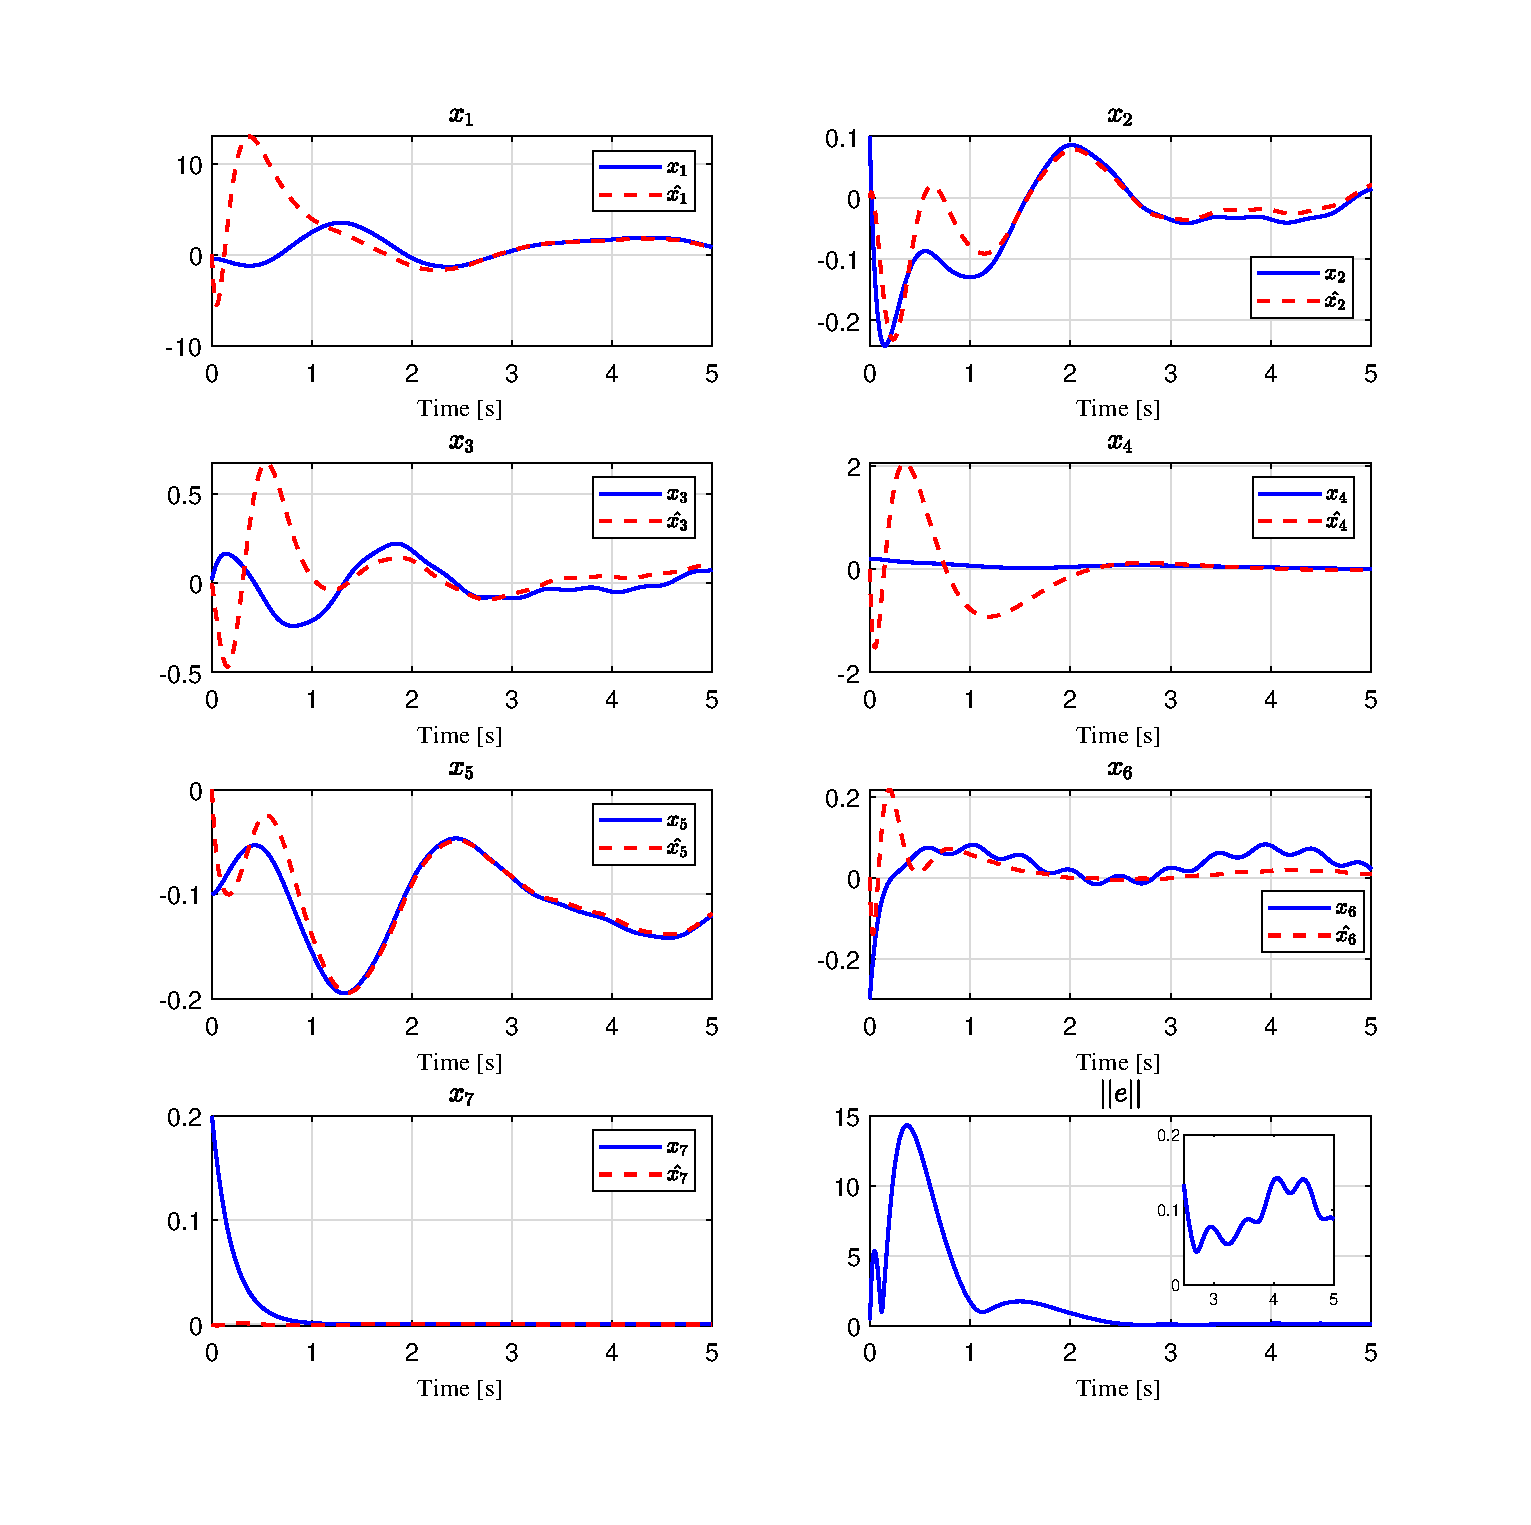
\includegraphics[width=17cm]{sys_7s_linear_states.eps}}
	\caption{Estimation of plant states $x_1,...,x_7$ and norm $\norm{e}$ with $d_0=d_{\infty}=0$.}
	\label{fig: CH4 Error states and norm, e_0 linear}
\end{figure}

\begin{figure}[htbp]
	\centering{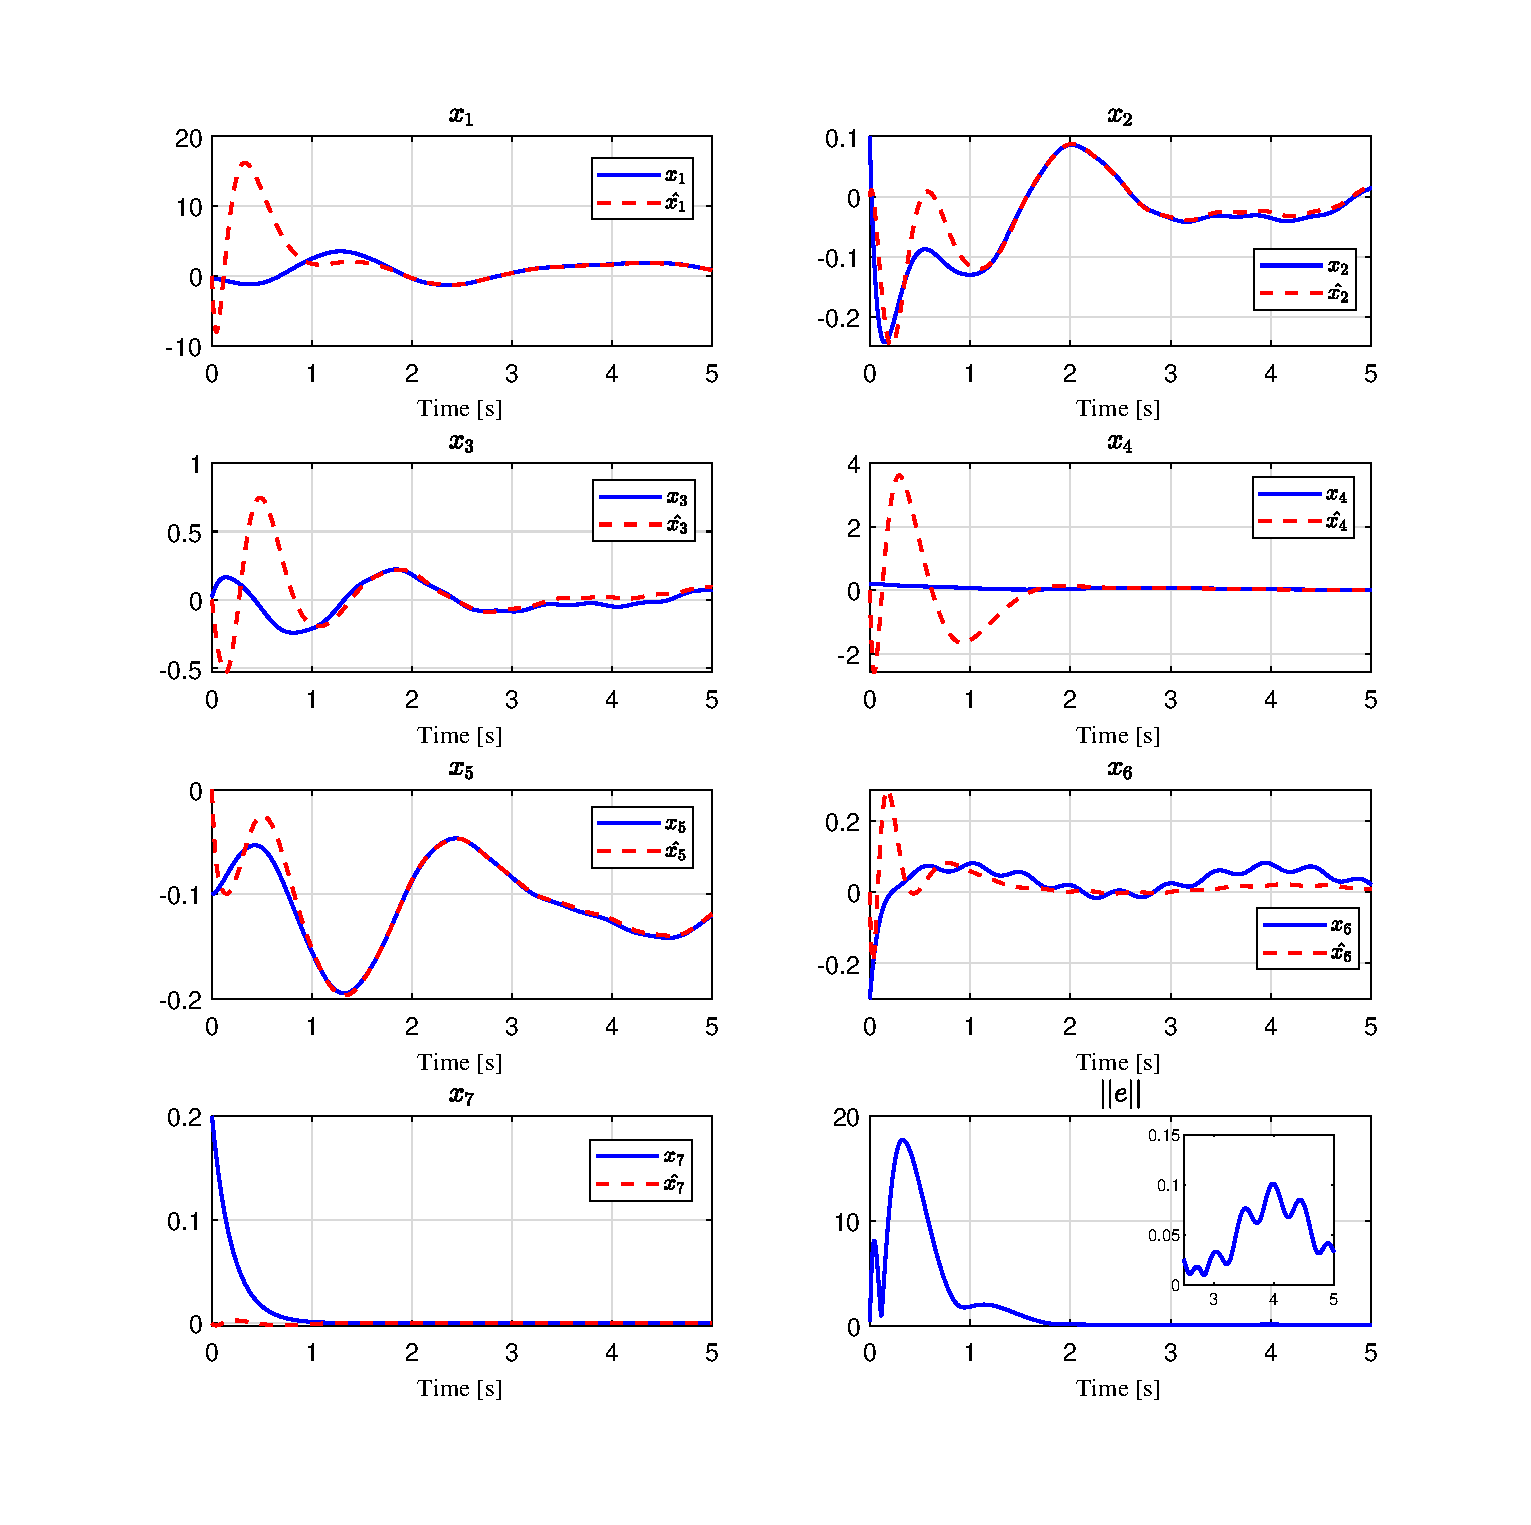
\includegraphics[width=17cm]{sys_7s_cont_states.eps}}
	\caption{Estimation of plant states $x_1,...,x_7$ and norm  $\norm{e}$ with $d_0=0,d_{\infty}=\tfrac{1}{9}$.}
	\label{fig: CH4 Error states and norm, e_0 cont}
\end{figure}

\begin{figure}[htbp]
	\centering{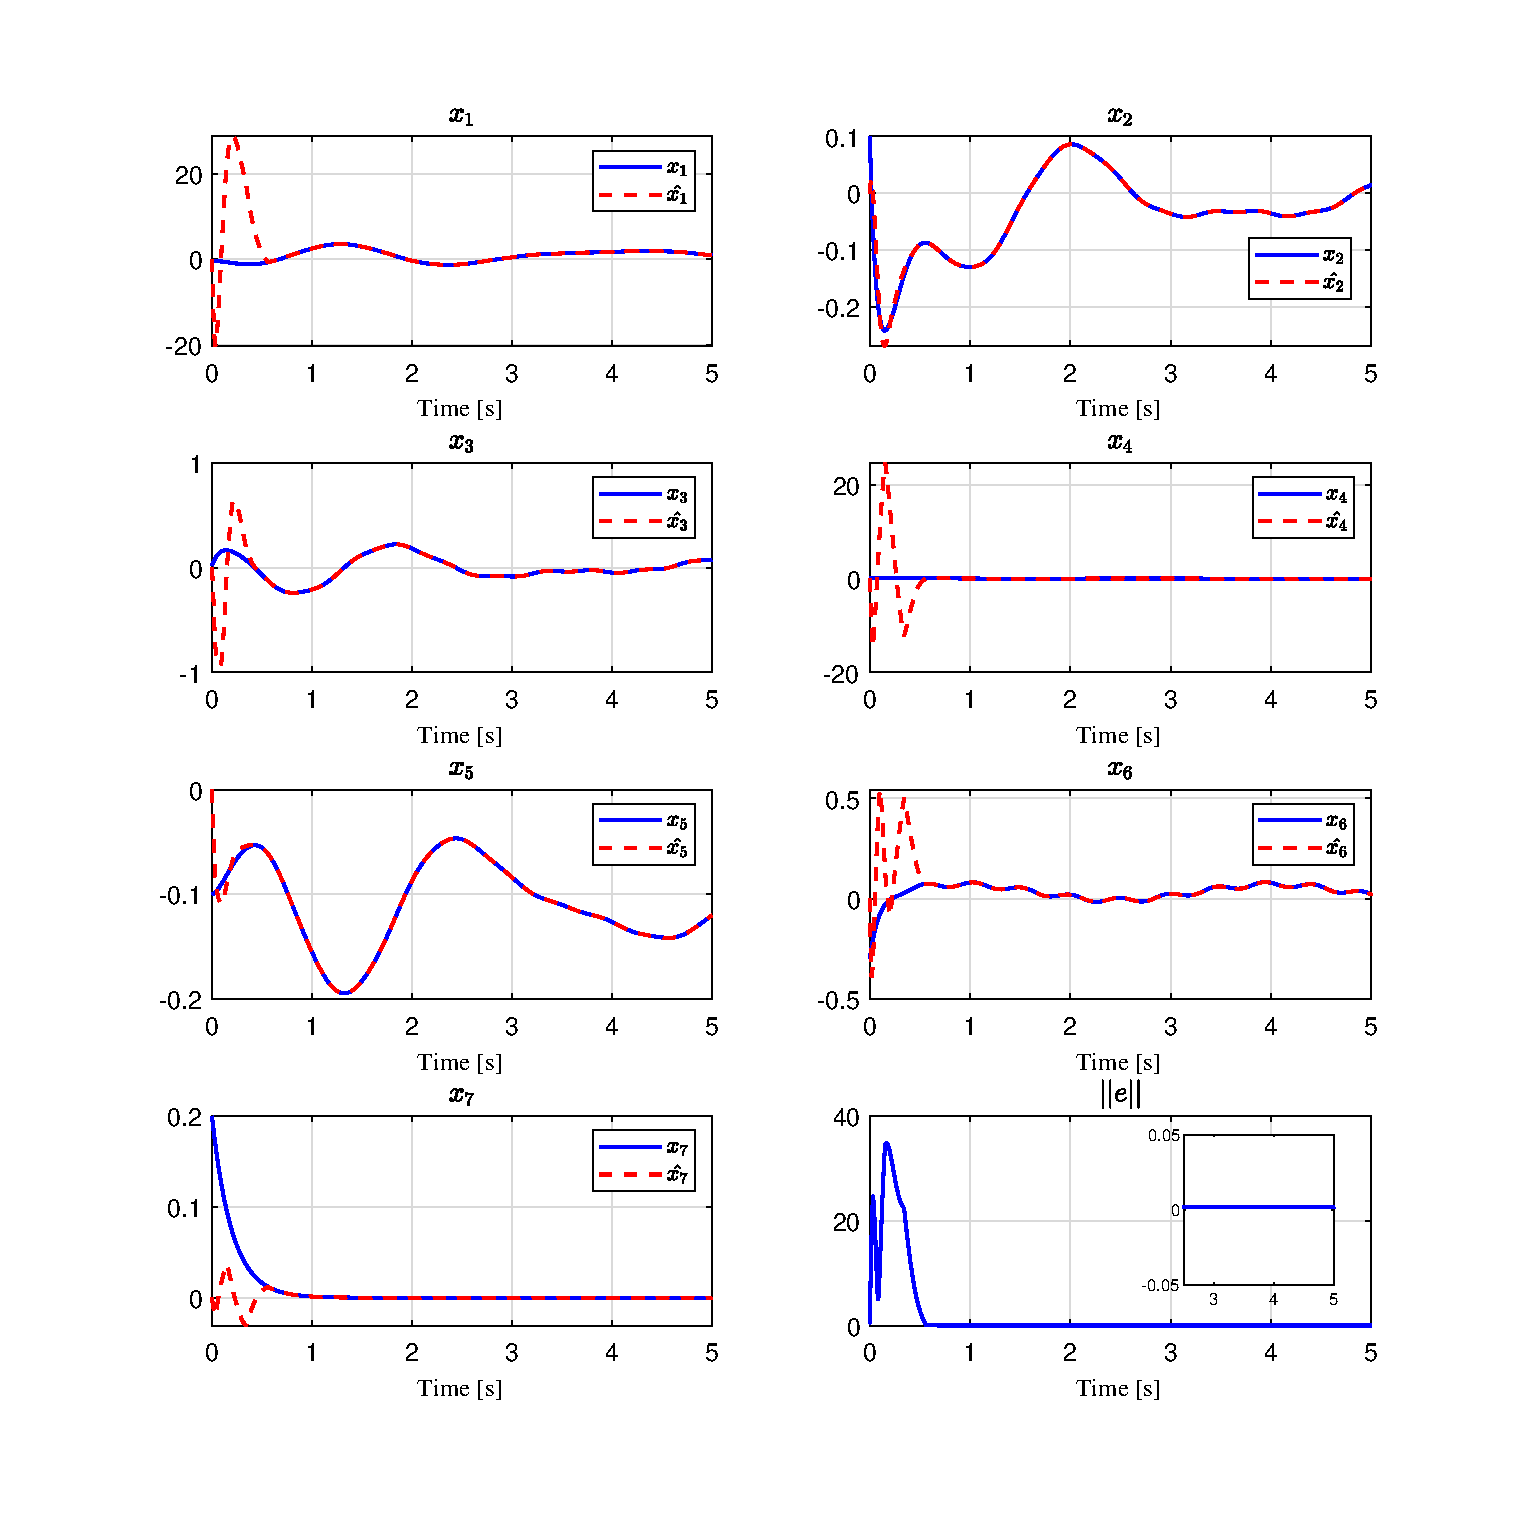
\includegraphics[width=17cm]{sys_7s_disc_states.eps}}
	\caption{Estimation of plant states $x_1,...,x_7$ and norm  $\norm{e}$ with $d_0=0,d_{\infty}=\tfrac{1}{9}$.}
	\label{fig: CH4 Error states and norm, e_0 disc}
\end{figure}

On the other hand, in the third case with $d_0=-1$ (discontinuous observer), the induced HOSM  allows the observer to compensate exactly the unknown inputs effect. It is shown in Figure \ref{fig: CH4 Error states and norm, e_0 disc}, that after 0.5s an exact convergence of the error norm to zero even in presence of unknown input is achieved, therefore, the states are estimated exactly in finite time.

In all cases, with appropriately gains selection the error converges to a neighborhood of zero in about one second but it is not clear what happens when the initial estimate is not close to the true state. For the third case, i.e. with $d_0=-1$, $d_{\infty}=\tfrac{1}{9}$ and setting now $L=5,\alpha=10$ we run a set of simulations, Figure \ref{fig: CH4 Error norm with orders} shows the norm of the error vector over a wide range orders of initial estimation error. Here, the error converge to zero in less than 4s for all cases.

In other words, we achieve more than finite-time, fixed-time stability of the estimation error, i.e. regardless of the initial magnitude of the error, the observer converges before certain time value $\bar{T}$, in this case we can see that the value of this upper cote of estimation time is $\bar{T}=4s$, but this can be reduced arbitrary by increasing appropriately the value of parameter $L$ as we said in the parameters tuning section.

\begin{figure}[htbp]
	\centering{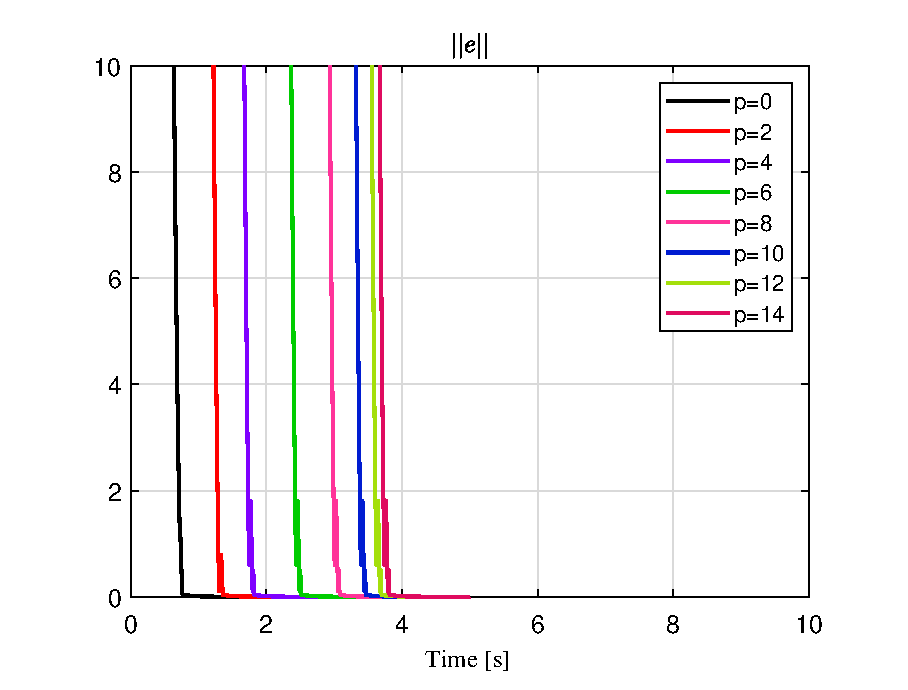
\includegraphics[width=10cm]{sys_7s_disc_FxT_error_orders.eps}}
	\caption{Norm of the estimation error $\norm{e}$ with different orders at initial error $e_0\times 10^p$ with $d_0=-1,d_{\infty}=\tfrac{1}{9}$.}
	\label{fig: CH4 Error norm with orders}
\end{figure}





	
		

	%====================================================================
	%                          Bibliografia
	%====================================================================
	\bibliographystyle{ieeetr}
	\bibliography{Citas}
\end{document}